\section{Authors and Readers in the \Gls{name} Ecosystem}

In the current incarnation of \glspl{name}, an author of code documentation writes a \gls{name} in order to adaptively describe  code programmers find while they browse the web.
A \gls{name} is an engine for generating explanations or demonstrations of code for a specific language, accessible as a simple web API.
When queried with the text of a web page, a \gls{name} detects explainable regions of the language, parses them, and returns explanations for each region as formatted HTML that can be viewed in a tooltip.

\begin{figure}
%%\centering
    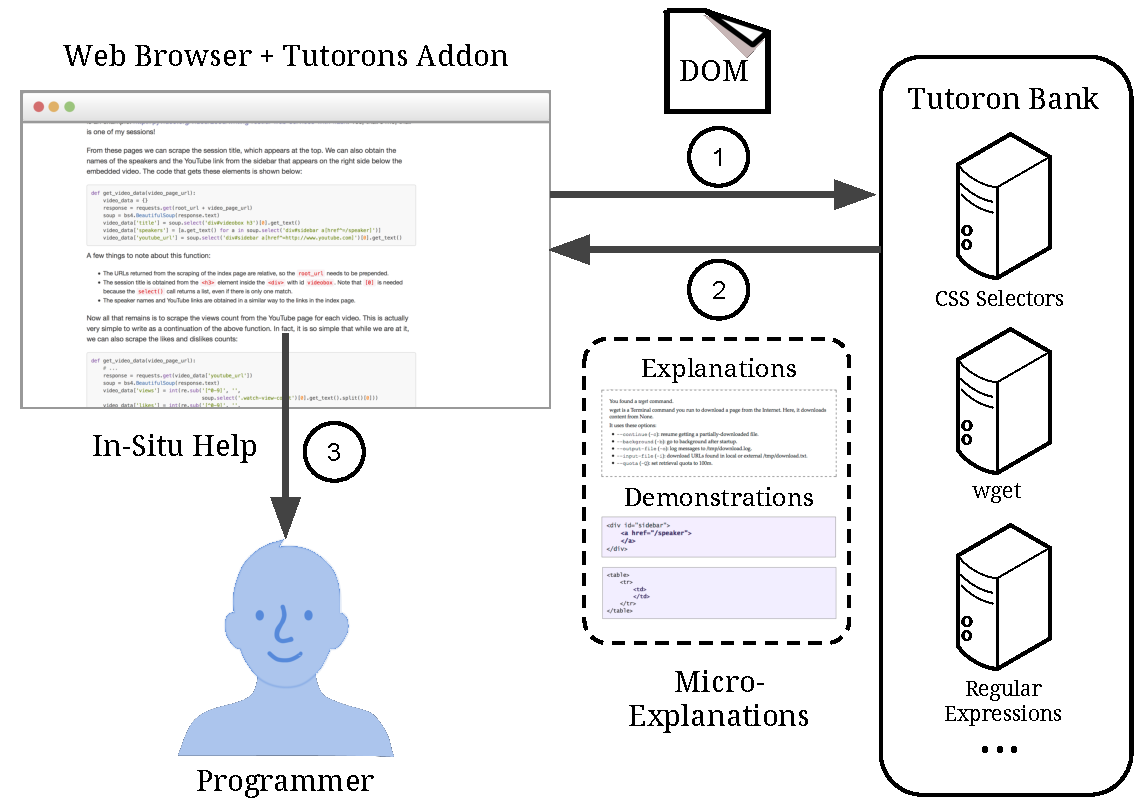
\includegraphics[width=\columnwidth]{figures/tutoron_ecosystem}
    \caption{
    The \Glspl{name} ecosystem and information flow.
    A programmer browses for help in a web browser with the \Glspl{name} addon.
    When she visits a page, the addon queries a bank of \gls{name} servers for different programming languages.
    Each server detects explainable regions of code and produces \glspl{exp}, or explanations and demonstrations of this code.
    The programmer can then view these in-situ and on-demand in tooltip-style overlays by simpling selecting explainable regions of code with the mouse.
    }
    \label{fig:tutoron_ecosystem}
\end{figure}

\if 0
\begin{figure}
\centering
    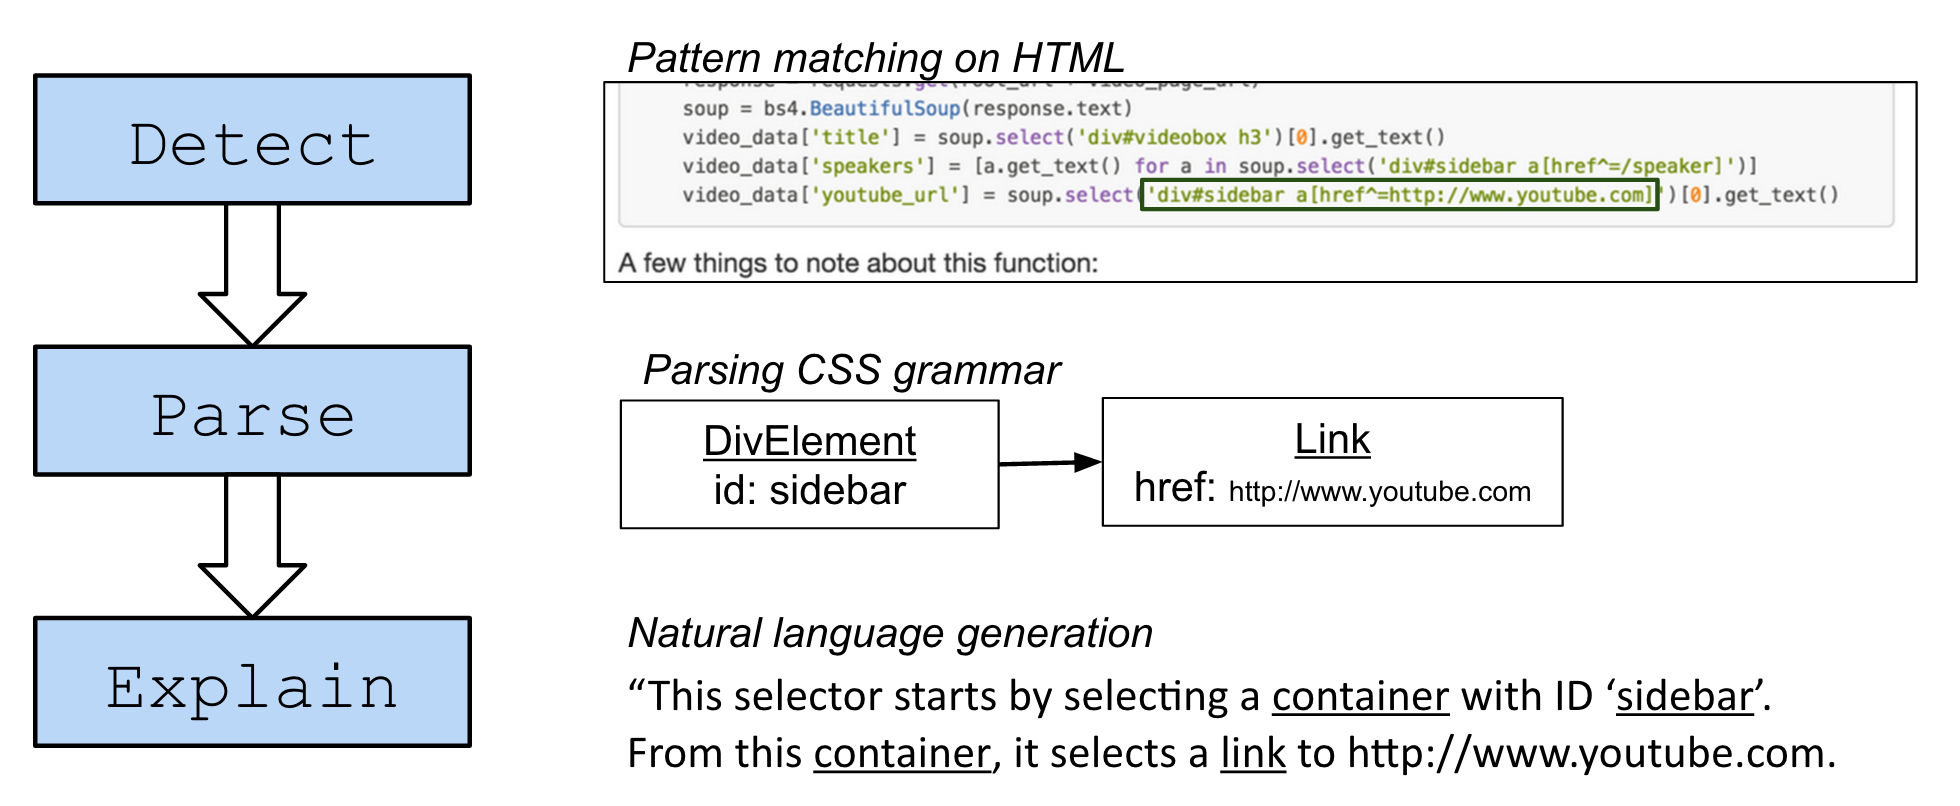
\includegraphics[width=\columnwidth]{figures/explanation_pipeline}
    \caption{\Glspl{name} \emph{detect} relevant code snippets, \emph{parse} them, and then \emph{generate explanations}.  Here we show examples of the output of each stage of the pipeline for a \gls{name} that explains CSS selectors.}
    \label{fig:explanation_pipeline}
\end{figure}
\fi

By installing an addon for the browser, a programmer receives instant access to \glspl{exp}, or in-situ descriptions of code found while browsing, from \gls{name} servers (Figure~\ref{fig:browser_tutorons_markup}).
The addon queries existing \glspl{name} with the page source, receiving micro-explanations for all explainable regions of code.
After receiving explanations, an explanation will appear in a tooltip overlaid on the document directly beneath the source any time the programmer selects an explainable string of text.
The \Glspl{name} addon can query many explanation servers for multi-language support within the same page.
The information flow of the \Glspl{name} ecosystem is shown in Figure~\ref{fig:tutoron_ecosystem}.
We note that our approach could work in other settings, e.g., as a Wordpress plugin, which would shift the burden of installing software from user to tutorial author.

The addon uses a \emph{push} method for fetching explanations rather than a \emph{pull} method, requesting for a server to detect all explainable instances of a language for a webpage.
This choice enables all explanations to be generated in a single batch when the user first accesses the page, reducing the load time to milliseconds instead of seconds to access explanations.
Each server is queried in parallel once the document is ready.
The original webpage is instantly available to the programmer, and \glspl{exp} for each language become available as each \gls{name} processes the DOM.
Computational burden resides on the server, dependent on the implementation.
Client procedures consists of string matching to explainable regions detected followed by insertion of generated HTML into a tooltip, which will be linear in time to the number of explanations.

By requiring \gls{name} servers to detect explainable regions, we resolve the problem where a user's selection may not cover a complete statement of the syntax of a language.
Pre-computing these explainable text regions, we can allow users to select explainable code with \emph{fuzzy boundaries} (see Figure~\ref{fig:fuzzy_boundaries}).
While our qualitative evaluations have shown that this selection mechanism is easy to use, we recognize the future efforts could improve usability.
This includes highlighting explainable regions in colors corresponding to each \gls{name} to indicate what code programmers can gain clarification on, and showing tooltips on hover or right-click events.

\begin{figure}
    \centering
    \framebox{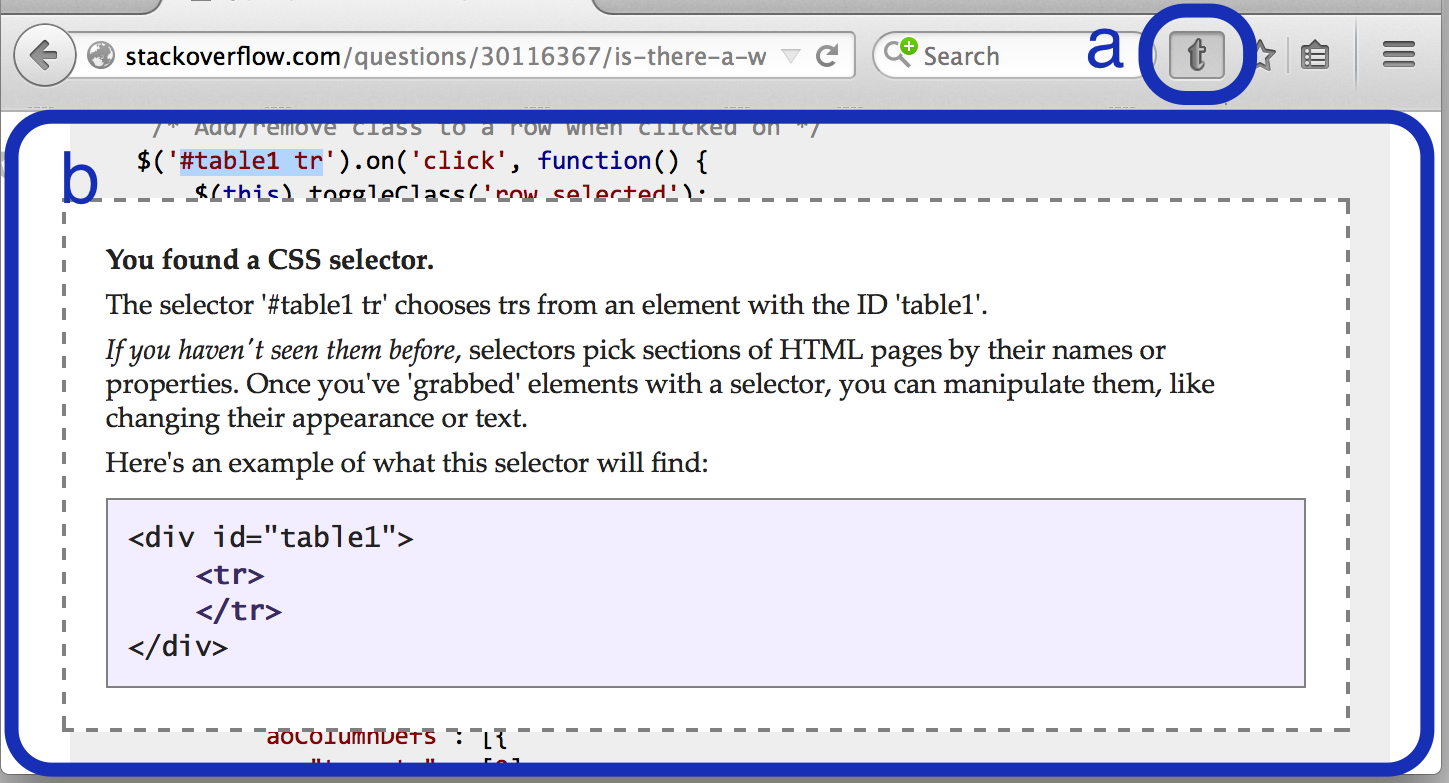
\includegraphics[width=\columnwidth]{figures/browser_tutorons_short}}
    \label{fig:browser_tutorons_markup}
    \caption{A user installs the \Glspl{name} addon.  \emph{(a)} Once she activates it, \emph{(b)} she can view automatically-generated, context-relevant explanations of code of supported languages in-situ while she browses programming help.}
\end{figure}

\begin{figure}
\centering{
    \subfigure[The CSS selector.]{
        \framebox{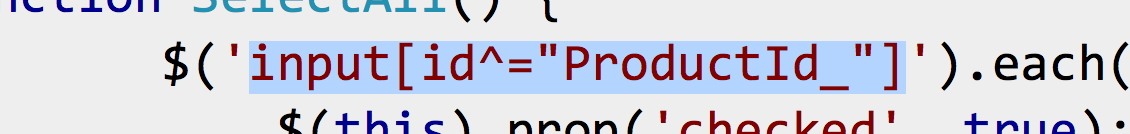
\includegraphics[width=.2\textwidth]{figures/selection_best}}
        \label{fig:selection_best}
    }
    \subfigure[The CSS selector with quotes.]{
        \framebox{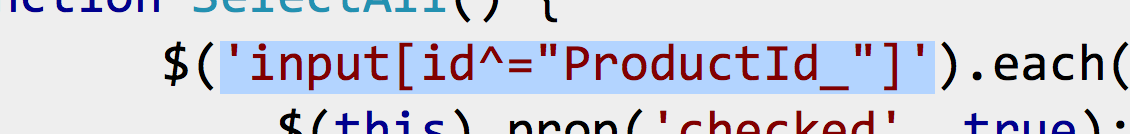
\includegraphics[width=.2\textwidth]{figures/selection_quotes}}
        \label{fig:selection_quotes}
    }
    \subfigure[A jQuery selection.]{
        \framebox{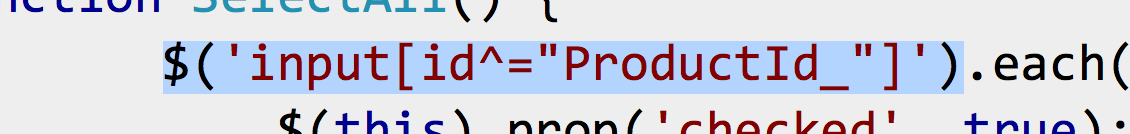
\includegraphics[width=.2\textwidth]{figures/selection_jquery}}
        \label{fig:selection_jquery}
    }
    \subfigure[A sloppy selection.]{
        \framebox{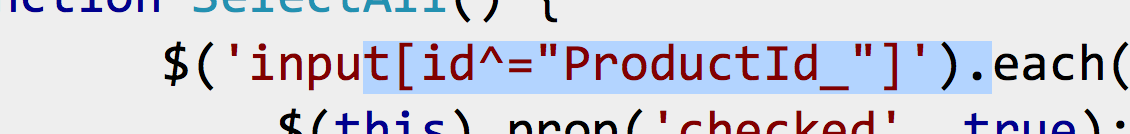
\includegraphics[width=.2\textwidth]{figures/selection_sloppy}}
        \label{fig:selection_sloppy}
    }
    \caption{
    The \Glspl{name} addon activates explanations for code when a user selects text.
    Explainable regions of code are detected on an explanation server and returned to the browser, where the addon enables users to view explanations with fuzzy selections.
    This lets them view \glspl{exp} without knowing the exact syntactic boundaries of the code they want to have described.
    }
    \label{fig:fuzzy_boundaries}
}
\end{figure}

\section{How to Build a \Gls{name}}

A \gls{name} is a routine that \emph{detects}, \emph{parses}, and \emph{explains} code for a specific language in HTML documents.
We describe each processing stage with overarching strategies we have determined for finding relevant code in a page, parsing languages, and generating domain-appropriate explanations.
We couch our discussion in the implementation details of two tutorons we developed for CSS selectors and the \texttt{wget} command and micro-expanations we generate for regular expressions.

\subsection{Detection}
In the \emph{detection} stage, a \gls{name} should extract explainable regions from an HTML document using the language's lexicon and / or syntax.
This can consist of four steps.

First, the \gls{name} extracts blocks of code from HTML pages by selecting code-related elements.
Our current tutorons extract bloks of code from \texttt{<code>} elements, though other common code elements are \texttt{<pre>} and formatted \texttt{<div>} elements.

Second, it divides code blocks into candidate explainable regions based on language-dependent rules.
CSS selectors and regular expressions can be detected as string literals in parsed Python or JavaScript code, requiring an initial parsing stage to detect these candidate regions.
Command lines like \texttt{wget} often occupy a line of a script, meaning that candidate regions can be found by splitting code blocks into lines.

Third, it passes candidate regions through a language-specific syntax checker to determine if it follows the grammar.
Note that if this can be combined with the parsing stage of the \gls{name} processing pipeline.

Finally, a \gls{name} may reduce false positives by filtering candidates to those containing tokens highly representative of the language.
This is necessary when candidate regions are small and the terminals of a grammar accept large character classes.
While the string \texttt{``marti''} in a JavaScript program could represent a custom HTML element we in a selector, it's really more likely a string for some other purpose --- elements in a CSS selector more often than not have tag names defined in the HTML specification (e.g., \texttt{p}, \texttt{div}, or \texttt{img}).

\subsection{Parsing}

Detected code snippets are parsed into a parse tree.
We have found two methods of building parsers to be useful.
When it is necessary to recognize a wide range of symbols and their semantics, \gls{name} authors can modify existing parsers, introducing hooks for extracting results of parsing.
Though this process can be highly involved, requiring a \gls{name} author to have access to the source code and for him to understand how to extract the information and exit the application safely at the appropriate time.
Ultimately, given the involved rules in parsing command lines, this was the right step to take for robust parsing of \texttt{wget} command lines.

However, in other cases, it may be appropriate to develop a custom parser for the language that supports a relevant subset of the language.
For CSS selectors, we wrote a parser in 30 lines of ANTLR\footnote{\url{www.antlr.org}}, which offered several benefits.
First, we had complete control over the parse tree produced.
As our explanations relied on parse tree traversal from leaf element through its parents, we constructed the tree in the format we wanted to traverse.
Second, our parser generator could create tree visitors in both Java and Python, which enabled us to traverse the tree in Java to leverage our natural language software and build example HTML using more familiar Python-based DOM manipulation libraries.
Custom parsers may also be necessary when parser code is too difficult to instrument to extract a useful parse tree, or when source code for the parser is not available.

\subsection{Explanation}

During the final stage, \emph{explanation}, the \gls{name} traverses the parse tree to generate explanations and demonstrations of the code.
The implementation details of this stage is specific to the structure of the parse tree and the ideal representation of the code.
In the next section, we describe techniques that we hope provide inspiration for future language-specific \glspl{exp}.